\begin{figure}[ht]
  \centering
  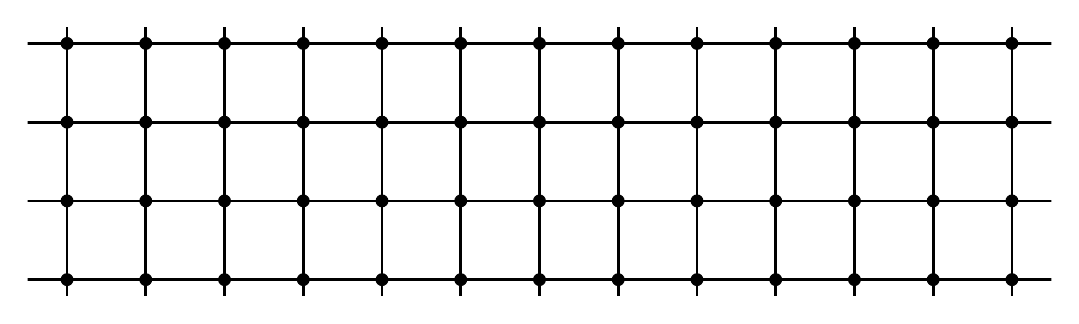
\begin{tikzpicture}
    \coordinate (Origin)   at (0,0);
    \coordinate (XAxisMin) at (-3,0);
    \coordinate (XAxisMax) at (5,0);
    \coordinate (YAxisMin) at (0,-2);
    \coordinate (YAxisMax) at (0,5);
    \begin{scope}
    \clip (-6.5,-0.2) rectangle (6.5,3.2);

    \foreach \x in {-6,-5,...,6}{% Two indices running over each
      \foreach \y in {0,1,...,6}{% node on the grid we have drawn 
        \draw[line width=1pt](\x-1,\y)--(\x+1,\y);
        \draw[line width=1pt](\x,\y-1)--(\x,\y+1);
        \node[draw,circle,inner sep=1.5pt,fill] at (\x,\y) {};
            % Places a dot at those points
      }
    }
    \end{scope} 
  \end{tikzpicture}
  \caption{O espaço $Cay(\mathbb{Z}^2, \{\pm(0, 1), \pm(0, 1) \})$.}
  \label{figure:cay(Z2)}
\end{figure}